\documentclass[/home/nkappler/Research/Dissertation/dissertation.tex]{subfiles}

\begin{document}
\begin{bibunit}
\chapter{Parasites in Dynamic Models of Food Web Biomass}

\begin{abstract}

The metabolic theory of ecology has produced many useful and compelling models
for ecosystem dynamics \cite{Yodzis1992, Williams2007, Molnar2012, Boit2012}. A
major strength of this theory is the observed allometric scaling of many key
biological properties, for example, the metabolic rate has been shown to be
highly dependent on body size \cite{Brown2004}. Existing dynamical models at
the ecosystem level do not account for parasite species. We show that a simple
method of incorporating parasites to the dynamical framework of the allometric
trophic network model decreases biomass, activity, and persistence for a range
of consumer resource body size ratios and fractions of parasites in the food
web. Despite the observed decreases in persistence, the model predicts that
coexistence of parasites and free livers is possible with simple dynamical
rules.

\end{abstract}

\newpage

\section{Introduction}

More than 40 years ago, Robert May showed that contemporary ecosystem models
were insufficient to explain the diversity observed in nature - that is,
diversity did not beget stability according to his model \cite{May1972}. The
challenge was leveled to ``elucidate the devious strategies which make for
stability in enduring natural systems.'' There are two major improvements to be
made to May's analysis. First, more realistic network structures can be
imposed. May used a matrix of random interactions as a first approximation to
Darwin's ``entangled bank.'' As noted in Chapter 3, much more realistic models
of food web structure exist, and in particular, when a body size hierarchy and
more realistic models of food web structure are used, May's dire predictions
are mitigated \cite{Allesina2012}. A second improvement can be made by
considering more realistic models of species abundance or biomass.
\cite{Boit2012} showed that the Allometric Trophic Network (ATN) model was able
to accurately capture the seasonal dynamics of a relatively complex aquatic
food web. However, parasites complicate both of the above findings; the
consumer - resource body size hierarchy was central to the results in
\cite{Allesina2012} and the empirical food web modeled in \cite{Boit2012} did
not include any parasitic taxa. 
 
Parasites have traditionally been modeled as pathogens within epidemiological
models; thus the disease, not the parasite itself was modeled \cite{May1991}.
Such models have not been incorporated into food web dynamics and represent
different mechanisms than found in the ATN model. We provide a baseline model
for incorporating parasitic taxa into the metabolic framework of the ATN model.
We test the ability of the proposed model to create persistent communities in
stochastically generated niche model food webs.

\section{Methods}

\subsection{Network Structures}

We simulate the ATN model on 100 niche models with species richness 40 and
connectance 0.15. We controlled the number of basal species by rejecting all
webs without exactly 6 basal species.  We controlled the number of parasites in
our food webs by switching the roles of certain consumers from free living
species to parasitic species. We chose which consumers to switch by first
randomly ordering all consumers. We then assigned the first fraction, $f_{par}$
of those species in the list to be parasites. In this way, parasites at low
levels of parasitism are also always parasites at higher levels of parasitism.
The same sequence of consumers was used for each simulation but each web
necessarily had a different sequence.  This allowed for direct comparisons
between models on each web. We used 9 different fractions of parasites,
corresponding to 1, 3, 5, ..., 17 parasites in each food web.

\subsection{Allometric Trophic Network Model}

The ATN model is an easily parameterized and extensible model that is capable
of reproducing realistic dynamics \cite{Boit2012}. At the heart of the ATN
model is the assumption that a species' metabolic rate controls both mortality
and biomass accumulation (unless otherwise noted the choices that follow can be
found in \cite{Brose2006b}). The dependence on this fundamental biological rate
along with empirically supported allometric scaling laws means that the only
species-specific parameter needed is body size \cite{Brown2004}. We use the
following formula to generate body sizes for any free living species in a niche
web:

\begin{equation}
    M_i= Z_{\!f}^{T_i-1}\label{eq:mFree}
\end{equation}

Where $T_i$ is the prey-averaged trophic level of species $i$ and $Z_{\!f}$ is
the average body size ratio of consumer $i$ to its prey items
\cite{Williams2004}. $Z_{\!f}$ will therefore determine the average body size
ratio of the entire food web. This means that a species at a given trophic
level will be $Z_{\!f}$ times larger than a species exactly one trophic level
lower. Note that this still allows for individual consumer-resource body size
ratios to vary for each species since we use prey-averaged trophic level. It is
not possible to define body sizes such that all links have the same
consumer-resource body size ratio for webs generated by the niche model. We ran
a full set of simulations for each of $Z_{\!f} = 10$ and $Z_{\!f} = 100$. 

Using the body size as defined in \eqref{eq:mFree}, we define the mass-specific metabolic rate as
\begin{equation}
x_i = a_{x_i} M_i^{-0.25}\label{eq:x}
\end{equation}

The $-0.25$ power has both empirical and theoretical support
(\cite{Brown2004, West1997}). The constant $a_{x_i}$ is the metabolic scaling
constant that varies across metabolic classes of species. In all simulations we
take $a_{x_i}=0.314$, which is the value for a broad collection of invertebrate
species. With these fundamental constants in hand we can write the following
dimensionless equations that govern the biomasses of all species in a food web
(see \cite{Yodzis1992} for the original 2-species derivation and
\cite{Williams2007} for an updated multi-species derivation): 
%Interaction of a_x_i with trophic level, metabolic classes, and body size
%ratios??

\begin{subequations}\label{eq:atn0}
\begin{align}
\frac{dB_{b}}{dt} &= r_bB_b\left(1-\frac{\sum_{k\in\text{basal}}B_k}{K}\right) - \sum_kx_kB_k\frac{y_{bk}F_{bk}}{e_{bk}}\label{subeq:basal0} \\ 
\frac{dB_{c}}{dt} &= -x_cB_c + x_cB_c\sum_ky_{kc}F_{kc} - \sum_k x_kB_k\frac{y_{ck}F_{ck}}{e_{ck}} \label{subeq:con0}
\end{align}
\end{subequations}

Here, $F_{ij}$ is a normalized functional response of $j$ preying on $i$. Note
that this functional response represents how the \textit{assimilation} of
biomass by a predator varies with changes in prey biomass (which has been shown
to vary allometrically, see \cite{Brown2004}), \textit{not} the consumption of
prey biomass. It has the following form:

\begin{equation}
    F_{ij} = \frac{\omega_{ij}B_j^{1+q}}{B_0^{1+q} + \sum_k\omega_{kj}B_k^{1+q}}\label{eq:fr0}
\end{equation}

In equation \ref{eq:fr0}, $q$ quantifies deviation from a multi-species type II
functional response; there is strong empirical support for $0<q<1$ in a wide
range of species interactions. $\omega_{ij}$ is the relative preference for
prey item $j$ by $i$ and $B_0$ is the half-saturation density. When $q=0$ and
$j$ has only one prey, $B_0$ is the density of prey that yields an attack rate
on $i$ by $j$ equal to half the maximum attack rate; it is related to the
handling time in more traditional formulations of type II functional responses
\cite{Holling1959}. In the case of multiple prey or $h\neq0$, $B_0$ is harder to
interpret but generally affects how quickly the functional response as a
function of prey biomass approaches its saturating value. In \eqref{eq:atn0},
$B_b$ and $B_c$ denote the biomass density of basal and consumer species,
respectively; thus \eqref{subeq:basal0} and \eqref{subeq:con0} represent rates
of change of basal and consumer populations, respectively (regardless of
whether the consumer is a free liver or parasite).  $r_b$ is the intrinsic
growth rate of basal species $b$ and $K$ is the community carrying capacity of
basal species. $x_i$ is the mass specific metabolic rate of consumer $i$.
$y_{ij}$ is the maximum assimilation rate of $i$ by $j$ relative to $j$'s
metabolic rate; $y_{ij}$ varies according to the metabolic class of the
consumer. $e_{ij}$ is the assimilation efficiency of $j$ when consuming $i$ and
varies according to the type of prey (autotroph or heterotroph prey item).  



\subsection{Introducing Parasites\label{subsec:paraIntro}}
 
 In this study, the most basic difference between a free living consumer and a
 parasitic consumer is the body size ratio of the parasite to its host species.
 On average, a parasitic species will be much smaller than its host, whereas a
 free living consumer will usually be much larger than its prey. The body sizes
 of parasitic species were determined using the following formula (note that $k
 = \log Z_{\!f}$ and $p$ is the (common) logarithm of the parasite-host body size
 ratio):

\begin{equation}
M_i = 10^{p + k(T_i - 2)} \label{eq:mPara}
\end{equation}

With this choice of body size, parasites will be on average $10^{p}$ times the
size of their free living hosts, $10^k$ times the size of their parasitic prey
(same as free livers on free livers, the red dashed links in figure
\ref{fig:bsrCartoon}), and $10^{p-2k}$ times the size of their free living
predators (the green dashed link in \ref{fig:bsrCartoon}. The last ratio
($10^{p-2k}$) is not ideal since it significantly increases the average body
size ratio of free living consumers. From the parasitic body sizes we derive
the parasitic mass-specific metabolic rate using equation \eqref{eq:x}. We ran
a full set of simulations with each of $p=-3$ and $p=-4$. A schematic of the
body size hierarchy defined by equations \eqref{eq:mPara} and \eqref{eq:mFree}
is given in figure \ref{fig:bsrCartoon}.
%TODO: think about how to reference the work I did on this.

\begin{figure}
    \includegraphics[width=\textwidth]{\DissertationDir/Chapter4/figures/png/diagram-BsrCartoon.png}
    \caption[Cartoon of body size ratios]{This figure shows the body size
    hierarchy when body sizes are defined according to equations
\eqref{eq:mPara} and \eqref{eq:mFree}. In this figure, the volume of the
spheres scale with the body size, and arrows denote biomass flow. The situation
in the model is also more complicated since we do allow fractional trophic
levels.\label{fig:bsrCartoon}} \end{figure}

\subsection{Models\label{subsec:models}}

As described in section \ref{subsec:paraIntro}, each web will be tested with
different average body size ratios: free livers will be on average 10 times
larger than their prey in one set of simulations and 100 times larger in
another set ($k=1$ and $k=2$, respectively); parasites will be on average 1,000
or 10,000 times smaller than their host ($p=-3$ and $p=-4$, respectively).
These two factors lead to 4 sets of simulations. For each combination of free
liver and parasitic average consumer-resource body size ratios, we tested two
models: a null model in which parasites are simply smaller-bodied species, and
a parasite model in which the evolution of parasite biomass follows slightly
different rules from free liver biomass.

\begin{figure}
    \centering
    \begin{minipage}{.45\textwidth}
    \centering
    \subcaption{Null Model \label{subfig:modelsa}}
    \includegraphics[width=.95\textwidth]{\DissertationDir/Chapter4/figures/extra/Null.png}%
\end{minipage}%
    \begin{minipage}{.45\textwidth}
    \centering
    \subcaption{Parasite Model\label{subfig:modelsb}}%
    \includegraphics[width=.95\textwidth]{\DissertationDir/Chapter4/figures/extra/Con+Ref.png}%
\end{minipage}%
\vspace{.2in}  
    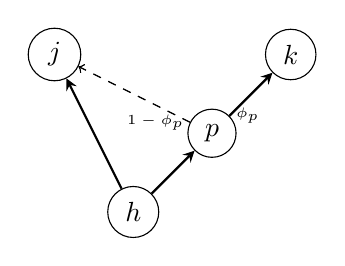
\begin{tikzpicture}
        \node[draw,circle] at (0,0) (j) {$j$};
        \node[draw,circle] at (1,-2) (h) {$h$};
        \node[draw,circle] at (2,-1) (p) {$p$};
        \node[draw,circle] at (3,0) (k) {$k$};
        \draw[->,>=stealth,thick] (h)--(j);
        \draw[->,>=stealth,thick] (h)--(p);
        \draw[->,>=stealth,thick] (p)-- node [pos = 0,anchor=west,inner sep =
            2pt] {\tiny $\phi_p$} (k);
        \draw[->,dashed] (p)--(j);
        \draw[->,dashed] (p) -- node [pos = 0,anchor=east,inner sep = 2pt]
            {\tiny $1-\phi_p$}(j) ;
    \end{tikzpicture}
    \subcaption{Parasite Model Schematic \label{fig:concDiagram}}
    \caption[Cartoon of dynamical models]{Figures
            \ref{subfig:modelsa} and \ref{subfig:modelsb} illustrate the
            differences between the two versions of ATN dynamics that were
            tested.  Figure \ref{fig:concDiagram} illustrates the parasite
            model. The fraction ($1-\phi_p$) of $p$'s biomass that is inside
            host $h$ is consumed when $h$ is concomittantly eaten by the host's
            consumer, $j$.  The fraction of $p$'s biomass that is outside of a
            host ($\phi_p$) is eaten by its predator, $k$.
    \label{fig:models}}
\end{figure}

%\begin{figure}
%\caption{Null Model\label{subfig:modelsa}}
%\includegraphics[width=.45\textwidth]{cartoon/Null.png}
%\end{figure}
%\begin{figure}
%\caption{refuge\label{subfig:modelsb}}
%\includegraphics[width=.45\textwidth]{cartoon/Null+Ref.png}
%\end{figure}
%
%\begin{figure}
%\caption{concomittant\label{subfig:modelsc}}
%\includegraphics[width=.45\textwidth]{cartoon/Null+Con.png}
%\end{figure}
%\begin{figure}
%\caption{refuge with concomittant\label{subfig:modelsd}}
%\includegraphics[width=.45\textwidth]{cartoon/Con+Ref.png}
%\end{figure}


In the null model (figure \ref{subfig:modelsa}), parasites are vulnerable to
their predators while both inside and outside their hosts and they are not
susceptible to concomittant predation. The only differences between a parasite
and free liver at the same trophic level in this model is their body sizes (and
metabolic rates). In the parasite model (figure \ref{subfig:modelsb}), we
introduce two changes. First, we introduce a parameter, $\phi_i$, to the null
model that controls the fraction of parasitic biomass outside of a host; this
can be considered a crude implementation of parasitic life stages. A parasite
is protected from trophic predation while inside its host.  We also add
concomittant predation of parasites within their hosts (see figure
\ref{fig:concDiagram}).

%\begin{figure}
%%This is a schematic for concomittant predation.
%    \centering
%%  \includegraphics[width=.3\textwidth]{\DissertationDir/Chapter4/figures/png/diagram-ConcomittantPredation.png}
%    \begin{tikzpicture}
%        \node[draw,circle] at (0,0) (j) {$j$};
%        \node[draw,circle] at (1,-2) (h) {$h$};
%        \node[draw,circle] at (2,-1) (p) {$p$};
%        \node[draw,circle] at (3,0) (k) {$k$};
%        \draw[->,>=stealth,thick] (h)--(j);
%        \draw[->,>=stealth,thick] (h)--(p);
%        \draw[->,>=stealth,thick] (p)-- node [pos = 0,anchor=west,inner sep =
%            2pt] {\tiny $\phi_p$} (k);
%        \draw[->,dashed] (p)--(j);
%        \draw[->,dashed] (p) -- node [pos = 0,anchor=east,inner sep = 2pt]
%            {\tiny $1-\phi_p$}(j) ;
%    \end{tikzpicture}
%    \caption[Diagram of Parasite model]{This diagram illustrates the parasite model. The fraction
%        ($1-\phi_p$) of $p$'s biomass that is inside host $h$ is consumed when
%        $h$ is concomittantly eaten by the host's consumer, $j$.  The fraction
%        of $p$'s biomass that is outside of a host ($\phi_p$) is eaten by its
%        predator, $k$.
%    \label{fig:concDiagram}}
%\end{figure}

In principle, the parameter $\phi_i$ could vary for each species in the  
parasite model. Since this was not a focus of the study we used a constant
fraction for all parasites and set $ \phi_i=1$ for free livers:

\begin{equation}
\phi_i = 
\left\{
\begin{array}{c c c}
\phi & \text{if} & i:\text{ parasite}\\
1 & \text{if} & i:\text{ free liver}\\
\end{array}\right.\label{eq:phi}
\end{equation}

The introduction of $\phi_i$ required significant changes to the ATN model
(equations \eqref{eq:atn1} and \eqref{eq:fr0}).


\begin{subequations}\label{eq:atn1}
\begin{align}
    \frac{dB_{b}}{dt} &= r_bB_b\left(1-\frac{\sum_{k\in\text{basal}}B_k}{K}\right) - \sum_k\phi_kB_kx_k\frac{y_{bk}^{}F_{bk}^{(troph)}}{e_{bk}} - \sum_k(1-\phi_k)B_kx_k\frac{y_{bk}^{}F^{(para)}_{bk}}{e_{bk}}\label{subeq:basal1} \\ 
    \frac{dB_{c}}{dt} &= -x_cB_c + \phi_cx_cB_c\sum_ky_{kc}^{ }F^{(troph)}_{kc} + (1-\phi_c)x_cB_c\sum_ky_{kc}^{ }F^{(para)}_{kc} \label{subeq:con1}\\ 
    & - \sum_k \phi_kx_kB_k\frac{y_{ck}^{}F^{(troph)}_{ck}}{e_{ck}} - \sum_k (1-\phi_k)x_kB_k\frac{y_{ck}^{}F^{(para)}_{ck}}{e_{ck}}\nonumber
\end{align}
\end{subequations}

Where the new functional responses are given by 

\begin{subequations}\label{eq:fr1}
\begin{align}F_{ij}^{(troph)} &= \frac{\omega_{ij}^{(troph)}(\phi_iB_i)^{1+q}}{B_0^{1+q} + \sum_k\omega^{(troph)}_{kj}(\phi_kB_k)^{1+q}} \label{subeq:fr1troph}\\
F_{ij}^{(para)} &= \frac{\omega_{ij}^{(para)}(\phi_iB_i)^{1+q}}{B_0^{1+q} + \sum_k\omega^{(para)}_{kj}(\phi_kB_k)^{1+q}} \label{subeq:fr1para}
\end{align}
\end{subequations}

The idea in equation \ref{eq:fr1} is to split the functional response according
to whether a link $i\to j$ represents predation or parasitism by $j$ on $i$. By
treating parasitism and trophic consumption links differently, we are
effectively treating the food web with parasites as a multiplex network. In the
case of predation (equation \eqref{subeq:fr1troph}), only the portion of $j$'s
biomass that is outside of a host can be a predator (hence the fraction
$\phi_c$ ahead of $F_{kc}^{(troph)}$ in equation \eqref{subeq:con1}).
Conversely, only the portion of biomass that is inside a host can be a parasite
(hence the fractions $(1-\phi_c)$ and $(1-\phi_k)$ in equations
\eqref{subeq:con1} and \eqref{subeq:basal1}).  Finally, a consumer (parasitic
or free living) will only consume and search for the portion of prey biomass
that is outside of hosts (hence the $\phi_j$ and $\phi_k$ in the numerator and
denominator, respectively, of equation \eqref{subeq:fr1troph}).  Thus, the
preference for a particular species is now determined by
$\omega_{ij}^{(troph)}$ in $F_{ij}^{(troph)}$ and $\omega_{ij}^{(para)}$ in
$F_{ij}^{(para)}$. These new preferences take into account the fact that a
parasite does not have to divide its foraging time as a free liver among its
hosts. By the same token, the parasite doesn't have to divide its 'foraging'
time among its free living (i.e. trophic) prey items when within a host.

The second addition is concomittant predation on parasites; this is included as
an additional term subtracted at the end of the consumer's growth rate
equation, \eqref{subeq:con1}. Note that this means we don't allow biomass
accumulation of concomittant predators from concomittant consumption of
parasite biomass. The term can be compactly expressed as \begin{equation} C_p =
\sum_ha_{ph}L_h \label{cp1} \end{equation} where $a_{ph}$ is the amount of
biomass of parasite $p$ per unit of biomass of host $h$, and $L_h$ is the total
trophic consumption (total rate of biomass loss due to predation by classic
consumers) of host $h$. We define $a_{ph}$ as the amount of biomass
accumulation by parasite $p$ from parasitism of host $h$ relative to the total
biomass accumulation by parasite $p$ from all of its hosts. The equation is 

\begin{equation}
    a_{ph} = \frac{(1-\phi_p)B_p}{B_h}\frac{y_{hp}^{}F_{hp}^{(para)}}{\sum_{k}y_{kp}^{}F^{(para)}_{kp}} \label{eq:aph1}
\end{equation}

Finally,

\begin{equation}
    L_h = \sum_kx_kB_k\frac{y^{}_{hk}F^{(troph)}_{hk}}{e^{}_{hk}} \label{eq:Th1}
\end{equation}

To summarize,

\begin{equation}
    C_p = \sum_h \left(\frac{(1-\phi_p)B_p}{B_h} \frac{y_{hp}^{}F^{(para)}_{hp}}{\sum_{k}y_{kp}^{}F^{(para)}_{kp}} \left[\sum_kx_kB_k\frac{y_{kh}^{}F^{(troph)}_{kh}}{e_{kh}^{}}\right]  \right) \label{eq:cp2}
\end{equation}

\subsection{Summary}


We ran each model on each food web with each combination of body sizes with 9
different fractions of parasites in each web, for a total of
$2\times4\times9\times 100 =7200$ simulations. We simulated the biomass
evolution of all 40 species in each web under each treatment using \verb|ode45|
in Matlab R2016b using an absolute error tolerance of $1\cdot10^{-16}$ and a
relative error tolerance of $1\cdot10^{-6}$. We also employed an in-the-loop
extinction threshold of $10^{-10}$ using the event detection feature of
Matlab's ode solver suite. As soon as the biomass of a species crossed the
threshold, we set its biomass equal to zero and removed it from the simulation.
This threshold was employed as a way to circumvent the ``atto-fox problem''
wherein unrealistically small population densities were able to persist and
later return to higher densities.


\pgfplotsset{table/search path=%
{\DissertationDir/Chapter4/data/figures-fullBreakdown}%
,compat=newest}
\fxnote{more figure references throughout}
\pgfplotstableset{col sep=comma} 

\newcommand{\curFig}{null}
\pgfkeys{/pgf/number format/.cd,zerofill} 

\section{Results} 
\fxnote[layout=index,target=structural comment]{Add another(similar section) with data on flows, link-level stuff} 
\fxwarning[layout=index,target=medium priority]{Relation btwn free and para
stats, i.e. corr. Plots..} 
\fxwarning[layout=index,target=medium priority]{Think about FINAL makeup of the web as well.} 

We analyze each model in turn; this section proceeds by showing results from
the null model and the parasite model separately. Throughout, we refer to
parasites with an average parasite-host \BSR~ of $10^{-3}$ as `large' and
parasites with an average parasite-host \BSR~ of $10^{-4}$ as `small'.

\subsection{Null Model} 

This section reports the results from the null model with different
predator-prey body-size ratios (BSRs) separately.

\subsubsection{Predator-Prey BSR of 10}

%Setting up:
\renewcommand{\curFig}{null-smallFree}
\pgfplotstableread{\curFig-bigPara}{\bigParaTab}
\pgfplotstableread{\curFig-smallPara}{\smallParaTab}
\pgfplotstablecreatecol[%
 expr = {\thisrow{yBioBasal}+\thisrow{yBioPara} + \thisrow{yBioFree}}%
                       ]{yBioTotal}{\bigParaTab} 


\pgfplotstablecreatecol[%
    expr = {\thisrow{yBioBasal}+\thisrow{yBioPara} + \thisrow{yBioFree}}
                       ]{yBioTotal}{\smallParaTab}


\begin{figure} 
    \centering {\large Null Model - Small Free-Livers}
    \includegraphics[width=\textwidth]{\DissertationDir//Chapter4/figures2//\graphicsExtension/null-smallFree.\graphicsExtension} 
    {%
        \phantomsubcaption{\label{fig:\curFig-a}}%
        \phantomsubcaption{\label{fig:\curFig-b}}%
        \phantomsubcaption{\label{fig:\curFig-c}}%
        \phantomsubcaption{\label{fig:\curFig-d}}%
        \phantomsubcaption{\label{fig:\curFig-e}}%
        \phantomsubcaption{\label{fig:\curFig-f}}%
        \phantomsubcaption{\label{fig:\curFig-g}}%
    }% 
    \caption[Dynamic results, Null model, Small free livers]{Figures \ref{fig:\curFig-a} and \ref{fig:\curFig-b} show 
        the average biomass distribution of basal, free living, and parasitic
        species in the null model with a predator-prey \aBSR~of 10 for both
        values of parasite-host \BSR~at each level of parasitism. Figures
        \ref{fig:\curFig-c} and \ref{fig:\curFig-d} show the average activities
        (metabolic rate $\times$ biomass) of all parasite and free living
        species, as well as the average primary production for the same models.
        Figures \ref{fig:\curFig-e} - \ref{fig:\curFig-g} show the
        corresponding persistences of all species (\ref{fig:\curFig-e}),
        free living species (\ref{fig:\curFig-f}), and parasitic species
        (\ref{fig:\curFig-g}), also at both parasite-host body-size
        ratios.\label{fig:null-smallFree}} 
\end{figure}

%Defining numbers for this sub-sub-section
\perChangeCol{\bigParaTab}{yBioTotal}{\bigBioPerDel}
\perChangeCol{\smallParaTab}{yBioTotal}{\smallBioPerDel}

\diffCol{\bigParaTab}{yBioFree}{\bigBioFreeDiff}
\diffCol{\smallParaTab}{yBioFree}{\smallBioFreeDiff}

\diffCol{\bigParaTab}{yBioTotal}{\bigBioTotalDiff}
\diffCol{\smallParaTab}{yBioTotal}{\smallBioTotalDiff}

\pgfmathparse{abs(\bigBioFreeDiff/\bigBioTotalDiff)*100}
\edef\bigBioFracBioDecFree{\pgfmathresult}

\pgfmathparse{abs(\smallBioFreeDiff/\smallBioTotalDiff)*100}
\edef\smallBioFracBioDecFree{\pgfmathresult}

\perChangeCol{\bigParaTab}{yBioPara}{\bigBioPerDelPara}
\pgfmathparse{\bigBioPerDelPara/100} \edef\bigBioPerDelPara{\pgfmathresult}

\perChangeCol{\smallParaTab}{yBioPara}{\smallBioPerDelPara}
\pgfmathparse{\smallBioPerDelPara/100} \edef\smallBioPerDelPara{\pgfmathresult}

\getEl{9}{yBioPara}\bigParaTab
\edef\bigMeanBioPara{\pgfplotsretval}

\getEl{9}{yBioPara}\smallParaTab
\edef\smallMeanBioPara{\pgfplotsretval}

\pgfmathparse{\bigMeanBioPara/\smallMeanBioPara}
\edef\bigSmallParaRatio{\pgfmathresult}

\perChangeCol{\bigParaTab}{yPerAll}{\bigParaPerRelChange}
\perChangeCol{\smallParaTab}{yPerAll}{\smallParaPerRelChange}

\perChangeCol{\bigParaTab}{yPerFree}{\bigParaPerRelChangeFree}
\perChangeCol{\smallParaTab}{yPerFree}{\smallParaPerRelChangeFree}

%Text:
%Figure \ref{fig:null-smallFree} shows the results of the null model with both
%parasite-host \aBSR s.  In figures \ref{fig:\curFig-a} and
%\ref{fig:\curFig-b}, we see a decrease in total biomass of
%\pn[precision=0]{\bigBioPerDel}\% and \pn[precision=0]{\smallBioPerDel}\% for
%webs with large and small parasites, respectively.  The majority of biomass
%decrease in absolute terms occurred in the free living species; the decrease in
%free living biomass accounted for \pn[precision=0]{\bigBioFracBioDecFree}\% and
%\pn[precision=0]{\smallBioFracBioDecFree}\% of the total biomass decrease in
%figures \ref{fig:\curFig-a} and \ref{fig:\curFig-b}, respectively.  The
%parasite biomass increased as the number of parasitic species increased,
%growing by factors of \pn[precision=1]{\bigBioPerDelPara} and
%\pn[precision=1]{\smallBioPerDelPara} in figures \ref{fig:\curFig-a} and
%\ref{fig:\curFig-b}, respectively. \fxnote{TODO: make data for per/species bio}

%Note also that there was significant variability in the mean biomass among
%webs at high
%levels of parasitism: the mean and standard deviation of \fxnote*{Check Total
%Biomass?}{free living biomass} \fxwarning{corr. btwn free\& para per. or bio?}
%at 50\% parasitism were \printFromTab{9}{yBioAll}{\bigParaTab}{precision=3}
%and \printFromTab{9}{sBioAll}{\bigParaTab}{precision=3} in figure
%\ref{fig:\curFig-a} and \printFromTab{9}{yBioAll}{\smallParaTab}{precision=3}
%and \printFromTab{9}{sBioAll}{\smallParaTab}{precision=3} in figure
%\ref{fig:\curFig-b}.  These numbers imply a considerable \fxnote*{skewed =
%median \& \%-iles? could easily show this plot}{right-skew} to the distribution
%of free living biomasses at high levels of parasitism. 

%\begin{tikzpicture}
%    \begin{axis}
%        \addplot table [x=x,y expr=\thisrow{yActCon}/\thisrow{yActAll}]
%            {\smallParaTab};
%        \addplot table [x=x,y expr=\thisrow{yActCon}/\thisrow{yActAll}]
%            {\bigParaTab};
%    \end{axis}
%\end{tikzpicture}


%The effect of decreasing the parasite-host \aBSR~ on mean biomass was subtle.
%The most striking difference was in total parasitic biomass.  At the highest
%levels of parasitism, webs with smaller parasites had on average
%\pn[precision=1]{\bigSmallParaRatio} times more parasitic biomass than webs
%with larger parasites.  The webs with larger parasites also saw a decrease in
%average biomass of basal species at higher levels of parasitism.
%
%The addition of parasites generally caused a decrease in average species
%persistence.  The average persistence of all species decreased by
%\pn[precision=0]{\bigParaPerRelChange}\% in webs with larger parasites (from
%\printFromTab{1}{yPerAll}{\bigParaTab}{precision=2} to
%\printFromTab{9}{yPerAll}{\bigParaTab}{precision=2}) and
%\pn[precision=0]{\smallParaPerRelChange}\% in webs with smaller parasites (from
%\printFromTab{1}{yPerAll}{\smallParaTab}{precision=2} to
%\printFromTab{9}{yPerAll}{\smallParaTab}{precision=2}).  Free living species
%also saw decreases in average persistence of
%\pn[precision=0]{\bigParaPerRelChangeFree}\% (from
%\printFromTab{1}{yPerFree}{\bigParaTab}{precision=2} to
%\printFromTab{9}{yPerFree}{\bigParaTab}{precision=2}) in webs with large
%parasites and \pn[precision=0]{\smallParaPerRelChangeFree}\% (from
%\printFromTab{1}{yPerFree}{\smallParaTab}{precision=2} to
%\printFromTab{9}{yPerFree}{\smallParaTab}{precision=2}) in webs with small
%parasites.  Parasite persistence was roughly constant for both parasite sizes,
%about 0.30 for large parasites and 0.18 for small parasites.  Apart from the
%difference in parasite persistence, parasite body size had little impact on persistence measures.

%Observations:
The total biomass decreased over the range of parasitism values by \perChangePrint{precision=0}{\bigParaTab}{yBioTotal}\% in webs with larger
parasites and \perChangePrint{precision=0}{\smallParaTab}{yBioTotal}\% in webs
with smaller parasites. Free living biomass decreased by
\perChangePrint{precision=0}{\smallParaTab}{yBioFree}\% in webs with smaller
parasites and \perChangePrint{precision=0}{\bigParaTab}{yBioFree}\% in webs
with larger parasites. Basal biomass was less affected, decreasing only
\perChangePrint{precision=0}{\smallParaTab}{yBioBasal}\% in webs with smaller
parasites and \perChangePrint{precision=0}{\bigParaTab}{yBioBasal}\% in webs
with larger parasites. Parasite biomass grew with increasing parasite fraction,
increasing by \perChangePrint{precision=0}{\smallParaTab}{yBioPara}\% and
\perChangePrint{precision=0}{\bigParaTab}{yBioPara}\% in webs with smaller
and larger parasites, respectively.

The total activity (metabolic rate $\times$ biomass $+$ basal production) also
decreased over the range of parasitism, falling
\perChangePrint{precision=0}{\bigParaTab}{yActAll}\% and
\perChangePrint{precision=0}{\smallParaTab}{yActAll}\% in webs with larger
and smaller parasites, respectively. However, this change was 
dominated by the decrease in basal productivity, which made up the majority
of the overall web activity and decreased by
\perChangePrint{precision=0}{\bigParaTab}{yActBasal}\% and
\perChangePrint{precision=0}{\smallParaTab}{yActBasal}\% in webs with larger
and smaller parasites, respectively. The total activity of all
consumers also decreased, though only by 
\perChangePrint{precision=0}{\bigParaTab}{yActCon}\% and
\perChangePrint{precision=0}{\smallParaTab}{yActCon}\% in webs with larger and
smaller parasites, respectively. Note that within the class of consumers,
the share of activity attributed to parasites increased over the range of
parasitism values, and the share of activity due to free livers decreased over
the range of parasitism values; this represents a much more balanced trade-off
than in figures \ref{fig:\curFig-a} and \ref{fig:\curFig-b}.

Overall persistence also decreased over the range of of parasitism, falling
\perChangePrint{precision=0}{\bigParaTab}{yPerAll}\% and
\perChangePrint{precision=0}{\smallParaTab}{yPerAll}\% over the range of
parasitism for webs with larger and smaller parasites, respectively. Basal
species never went extinct, which means the decrease in persistence was driven
by free liver and parasite species extinctions. Free liver persistence fell by
\perChangePrint{precision=0}{\bigParaTab}{yPerFree}\% and
\perChangePrint{precision=0}{\smallParaTab}{yPerFree}\% over the range of
parasitism in webs with larger and smaller parasites, respectively. Parasite
persistence was on average low and fairly constant across all levels of
parasitism, staying near \printFromTab{4}{yPerPara}{\bigParaTab}{precision=2}
and \printFromTab{4}{yPerPara}{\smallParaTab}{precision=2} in webs with
larger and smaller parasites, respectively.


\subsubsection{Predator-Prey BSR of 100} 
%Setting up.
\renewcommand{\curFig}{null-bigFree}
\pgfplotstableread{\curFig-bigPara}{\bigParaTab}
\pgfplotstableread{\curFig-smallPara}{\smallParaTab}
\pgfplotstablecreatecol[%
    expr = {\thisrow{yBioBasal} + \thisrow{yBioPara} + \thisrow{yBioFree}}%
    ] {yBioTotal}{\bigParaTab} 
\pgfplotstablecreatecol[%
    expr = {\thisrow{yBioBasal} + \thisrow{yBioPara} + \thisrow{yBioFree}}%
    ] {yBioTotal}{\smallParaTab}

\begin{figure} 
    \centering {\large Null Model - Large Free-Livers}
    \includegraphics[width=\textwidth]{\DissertationDir//Chapter4/figures2//\graphicsExtension/null-bigFree.\graphicsExtension}%
    {%
         \phantomsubcaption{\label{fig:\curFig-a}}%
         \phantomsubcaption{\label{fig:\curFig-b}}%
         \phantomsubcaption{\label{fig:\curFig-c}}%
         \phantomsubcaption{\label{fig:\curFig-d}}%
         \phantomsubcaption{\label{fig:\curFig-e}}%
         \phantomsubcaption{\label{fig:\curFig-f}}%
         \phantomsubcaption{\label{fig:\curFig-g}}%
     }%
     \caption[Dynamic results, null model, large free livers]{Figures \ref{fig:\curFig-a} and \ref{fig:\curFig-b} show 
        the average biomass distribution of basal, free living, and parasitic
        species in the null model with a predator-prey \aBSR~of 10 for both
        values of parasite-host \BSR~at each level of parasitism. Figures
        \ref{fig:\curFig-c} and \ref{fig:\curFig-d} show the average activities
        (metabolic rate $\times$ biomass) of all parasite and free living
        species, as well as the average primary production for the same models.
        Figures \ref{fig:\curFig-e} - \ref{fig:\curFig-g} show the
        corresponding persistences of all species (\ref{fig:\curFig-e}),
        free living species (\ref{fig:\curFig-f}), and parasitic species
        (\ref{fig:\curFig-g}), also at both parasite-host body-size
        ratios.\label{fig:null-bigFree}} 
\end{figure}

%Numbers for this section
\perChangeCol{\bigParaTab}{yBioTotal}{\bigBioPerDel}
\perChangeCol{\smallParaTab}{yBioTotal}{\smallBioPerDel}

\diffCol{\bigParaTab}{yBioFree}{\bigBioFreeDiff}
\diffCol{\smallParaTab}{yBioFree}{\smallBioFreeDiff}

\diffCol{\bigParaTab}{yBioTotal}{\bigBioTotalDiff}
\diffCol{\smallParaTab}{yBioTotal}{\smallBioTotalDiff}

\pgfmathparse{abs(\bigBioFreeDiff/\bigBioTotalDiff)*100}
\edef\bigBioFracBioDecFree{\pgfmathresult}

\pgfmathparse{abs(\smallBioFreeDiff/\smallBioTotalDiff)*100}
\edef\smallBioFracBioDecFree{\pgfmathresult}

\perChangeCol{\bigParaTab}{yBioPara}{\bigBioPerDelPara}
\pgfmathparse{\bigBioPerDelPara/100} \edef\bigBioPerDelPara{\pgfmathresult}

\perChangeCol{\smallParaTab}{yBioPara}{\smallBioPerDelPara}
\pgfmathparse{\smallBioPerDelPara/100} \edef\smallBioPerDelPara{\pgfmathresult}

\getEl{9}{yBioPara}\bigParaTab \edef\bigMeanBioPara{\pgfplotsretval}

\getEl{9}{yBioPara}\smallParaTab \edef\smallMeanBioPara{\pgfplotsretval}

\pgfmathparse{\bigMeanBioPara/\smallMeanBioPara}
\edef\bigSmallParaRatio{\pgfmathresult}

\perChangeCol{\bigParaTab}{yPerAll}{\bigParaPerRelChange}
\perChangeCol{\smallParaTab}{yPerAll}{\smallParaPerRelChange}

\perChangeCol{\bigParaTab}{yPerFree}{\bigParaPerRelChangeFree} \perChangeCol{\smallParaTab}{yPerFree}{\smallParaPerRelChangeFree}

\perChangeCol{\bigParaTab}{yPerPara}{\bigParaPerChangePara}
\perChangeCol{\smallParaTab}{yPerPara}{\smallParaPerChangePara}

%Text
%Figure \ref{fig:null-bigFree} shows the results of the null model with both
%parasite-host \aBSR s.  We immediately see a decrease in total biomass of
%\pn[precision=0]{\bigBioPerDel}\% and \pn[precision=0]{\smallBioPerDel}\% for
%webs with large and small parasites, respectively. The majority of biomass
%decrease in absolute terms still occurred in the free living species; the
%decrease in free living biomass accounted for
%\pn[precision=0]{\bigBioFracBioDecFree}\% and
%\pn[precision=0]{\smallBioFracBioDecFree}\% of the total biomass decrease in
%figures \ref{fig:\curFig-a} and \ref{fig:\curFig-b}, respectively. The parasite
%biomass increased as the number of parasitic species increased, growing by
%factors of \pn[precision=1]{\bigBioPerDelPara} and
%\pn[precision=1]{\smallBioPerDelPara} in figures \ref{fig:\curFig-a} and
%\ref{fig:\curFig-b}, respectively.  Another striking feature not present in the
%biomass results with smaller free livers was a plateau in total biomass from
%roughly $20$\% parasitism to $35$\% parasitism.
% 
%Note also that there was significant variability in the mean biomass among
%food webs at all
%levels of parasitism: the mean and standard deviation of \fxnote*{Check Total
%Biomass? }{free living biomass} \fxwarning{corr. btwn free \& para bio or
%per.?} at $2.5$\% parasitism were
%\printFromTab{1}{yBioFree}{\bigParaTab}{precision=3} and
%\printFromTab{1}{sBioFree}{\bigParaTab}{precision=3} for figure
%\ref{fig:\curFig-a} and \printFromTab{1}{yBioFree}{\smallParaTab}{precision=3}
%and \printFromTab{1}{sBioFree}{\smallParaTab}{precision=3} for figure
%\ref{fig:\curFig-b}. The corresponding numbers at $50$\% parasitism were
%\printFromTab{9}{yBioFree}{\bigParaTab}{precision=3} and
%\printFromTab{9}{sBioFree}{\bigParaTab}{precision=3} for figure
%\ref{fig:\curFig-a} and \printFromTab{9}{yBioFree}{\smallParaTab}{precision=3}
%and \printFromTab{9}{sBioFree}{\smallParaTab}{precision=3} for figure
%\ref{fig:\curFig-b}. These numbers imply a considerable right-skew to the
%distribution of free living biomasses which worsened with increasing numbers of
%parasites.
%
%The effect of decreasing the parasite-host again had only slight effects \aBSR~
%on mean biomass.  The most striking difference was in total parasitic biomass:
%at the highest levels of parasitism, webs with smaller parasites had on average
%\pn[precision=1]{\bigSmallParaRatio} times more parasitic biomass than webs
%with webs with larger parasites. The webs with larger parasites also saw a
%decrease in average biomass of basal species at higher levels of parasitism.
%
%The addition of parasites generally caused a decrease in average species
%persistence, though the effect was not as strong as in webs with smaller
%free livers. The average persistence of all species decreased by
%\pn[precision=0]{\bigParaPerRelChange}\% with larger parasites (from
%\printFromTab{1}{yPerAll}{\bigParaTab}{precision=2} to
%\printFromTab{9}{yPerAll}{\bigParaTab}{precision=2}) and
%\pn[precision=0]{\smallParaPerRelChange}\% with smaller parasites (from
%\printFromTab{1}{yPerAll}{\smallParaTab}{precision=2} to
%\printFromTab{9}{yPerAll}{\smallParaTab}{precision=2}). Free living species
%also saw decreases in average persistence of
%\pn[precision=0]{\bigParaPerRelChangeFree}\% (from
%\printFromTab{1}{yPerFree}{\bigParaTab}{precision=2} to
%\printFromTab{9}{yPerFree}{\bigParaTab}{precision=2}) in webs with large
%parasites and \pn[precision=0]{\smallParaPerRelChangeFree}\% (from
%\printFromTab{1}{yPerFree}{\smallParaTab}{precision=2} to
%\printFromTab{9}{yPerFree}{\smallParaTab}{precision=2}) in webs with small
%parasites. Parasites saw an increase in persistence as parasite fractions
%increased from 2.5\% to 30\%, and remained roughly constant from 30\%
%parasitism to 50\% parasitism. Parasite persistence in webs with larger
%parasites increased \pn[precision=0]{\bigParaPerChangePara}\%  (from
%\printFromTab{1}{yPerPara}{\bigParaTab}{precision=2} to
%\printFromTab{7}{yPerPara}{\bigParaTab}{precision=2}) as parasitism increased
%from 2.5\% to 30\%; parasite persistence in webs with smaller parasites
%increased \pn[precision=0]{\smallParaPerChangePara}\%  (from
%\printFromTab{1}{yPerPara}{\smallParaTab}{precision=2} to
%\printFromTab{7}{yPerPara}{\smallParaTab}{precision=2}) over the same range of
%parasitism. 

%Observations:
The total biomass decreased over the range of parasitism values by
\perChangePrint{precision=0}{\bigParaTab}{yBioTotal}\% in webs with larger
parasites and \perChangePrint{precision=0}{\smallParaTab}{yBioTotal}\% in webs
with smaller parasites. Free living biomass decreased by
\perChangePrint{precision=0}{\smallParaTab}{yBioFree}\% in webs with smaller
parasites and \perChangePrint{precision=0}{\bigParaTab}{yBioFree}\% in webs
with larger parasites. Basal biomass was less affected, decreasing only
\perChangePrint{precision=0}{\smallParaTab}{yBioBasal}\% in webs with smaller
parasites and \perChangePrint{precision=0}{\bigParaTab}{yBioBasal}\% in webs
with larger parasites. Parasite biomass grew substantially with increasing
parasite fraction, increasing by
\perChangePrint{precision=0}{\smallParaTab}{yBioPara}\% and
\perChangePrint{precision=0}{\bigParaTab}{yBioPara}\% in webs with smaller and
larger parasites, respectively.

The total activity remained very close to the original value of
\printFromTab{1}{yActAll}{\bigParaTab}{precision=2} in webs with larger
parasites. Webs with smaller parasites experienced a
\perChangePrint{precision=0}{\smallParaTab}{yActAll}\% decrease in total
activity. Once again, we note the trade-off between free living and parasitic
activity resulting nearly the same consumer activity across all levels of
parasitism.

Overall persistence also decreased over the range of of parasitism, falling
\perChangePrint{precision=0}{\bigParaTab}{yPerAll}\% and
\perChangePrint{precision=0}{\smallParaTab}{yPerAll}\% over the range of
parasitism for webs with larger and smaller parasites, respectively. As before,
basal species never went extinct, so the decrease in persistence was again
driven by free liver and parasite species extinctions. Free liver persistence
fell by \perChangePrint{precision=0}{\bigParaTab}{yPerFree}\% and
\perChangePrint{precision=0}{\smallParaTab}{yPerFree}\% over the range of
parasitism in webs with larger and smaller parasites, respectively. Parasite
persistence was on average low and fairly constant across all levels of
parasitism, staying near \printFromTab{4}{yPerPara}{\bigParaTab}{precision=2}
and \printFromTab{4}{yPerPara}{\smallParaTab}{precision=2} in webs with larger
and smaller parasites, respectively.

\subsubsection{Effect of Free-Living Body Size}
The most striking difference between webs with larger and smaller free livers
is that webs with larger free livers have roughly 2 to 3 times as much biomass
as webs with smaller free livers. Webs with larger free livers also exhibited 
a smaller decrease in persistence of free living species than webs with smaller
free livers. Thus, although webs with larger free livers had noticeably lower
free liver persistence at 2.5\% parasitism, at 50\% parasitism, free living body
size had a much smaller effect on free liver persistence. The persistence of
parasite species showed markedly different behavior between webs with the two
different free liver body sizes. Webs with larger free livers saw a slight
increase in parasite persistence with increasing levels of parasitism; these
webs had very low parasite persistence at 2.5\% parasitism, and parasite
persistence that was comparable to that seen in webs with smaller free lives at
30\% and higher parasitism.


\subsection{Parasite Model} 
This section reports results from the full model with different predator-prey
body size ratios (BSRs) separately. 

\subsubsection{Predator-Prey Body Size Ratio of 10}
%Setting Up
\renewcommand{\curFig}{full-smallFree}
\pgfplotstableread{\curFig-bigPara}{\bigParaTab}
\pgfplotstableread{\curFig-smallPara}{\smallParaTab}
\pgfplotstablecreatecol[%
    expr = {\thisrow{yBioBasal} + \thisrow{yBioPara} + \thisrow{yBioFree}}%
    ] {yBioTotal}{\bigParaTab} 
\pgfplotstablecreatecol[%
    expr = {\thisrow{yBioBasal} + \thisrow{yBioPara} + \thisrow{yBioFree}}%
    ] {yBioTotal}{\smallParaTab}



\begin{figure} 
    \centering {\large Parasite Model - Small Free-Livers}
    \includegraphics[width=\textwidth]{\DissertationDir//Chapter4/figures2//\graphicsExtension/full-smallFree.\graphicsExtension} 
    {%
        \phantomsubcaption{\label{fig:\curFig-a}}%
        \phantomsubcaption{\label{fig:\curFig-b}}%
        \phantomsubcaption{\label{fig:\curFig-c}}%
        \phantomsubcaption{\label{fig:\curFig-d}}%
        \phantomsubcaption{\label{fig:\curFig-e}}%
        \phantomsubcaption{\label{fig:\curFig-f}}%
        \phantomsubcaption{\label{fig:\curFig-g}}%
    } 
    \caption[Dynamic results, parasite model, small free livers]{Figures \ref{fig:\curFig-a} and \ref{fig:\curFig-b} show the
        average biomasses of all basal, free living, and parasitic species in
        the full model with a predator-prey \aBSR~of 10 for both values of
        parasite-host \BSR. Figures \ref{fig:\curFig-c} and \ref{fig:\curFig-d}
        show the corresponding average activities and figures
        \ref{fig:\curFig-e} - \ref{fig:\curFig-g} show the persistences of all
        species (\ref{fig:\curFig-e}), free living species
        (\ref{fig:\curFig-f}), and parasitic species (\ref{fig:\curFig-g}),
        also at both parasite-host body-size ratios.\label{fig:full-smallFree}}
    \end{figure}

%Numbers for this section
\perChangeCol{\bigParaTab}{yBioTotal}{\bigBioPerDel}
\perChangeCol{\smallParaTab}{yBioTotal}{\smallBioPerDel}


\diffCol{\bigParaTab}{yBioFree}{\bigBioFreeDiff}
\diffCol{\smallParaTab}{yBioFree}{\smallBioFreeDiff}

\diffCol{\bigParaTab}{yBioTotal}{\bigBioTotalDiff}
\diffCol{\smallParaTab}{yBioTotal}{\smallBioTotalDiff}

\pgfmathparse{abs(\bigBioFreeDiff/\bigBioTotalDiff)*100}
\edef\bigBioFracBioDecFree{\pgfmathresult}

\pgfmathparse{abs(\smallBioFreeDiff/\smallBioTotalDiff)*100}
\edef\smallBioFracBioDecFree{\pgfmathresult}

\perChangeCol{\bigParaTab}{yBioPara}{\bigBioPerDelPara}
\pgfmathparse{\bigBioPerDelPara/100} \edef\bigBioPerDelPara{\pgfmathresult}

\perChangeCol{\smallParaTab}{yBioPara}{\smallBioPerDelPara}
\pgfmathparse{\smallBioPerDelPara/100} \edef\smallBioPerDelPara{\pgfmathresult}

\getEl{9}{yBioPara}\bigParaTab \edef\bigMeanBioPara{\pgfplotsretval}

\getEl{9}{yBioPara}\smallParaTab \edef\smallMeanBioPara{\pgfplotsretval}

\pgfmathparse{\bigMeanBioPara/\smallMeanBioPara}
\edef\bigSmallParaRatio{\pgfmathresult}

\edef\smallFreeBigParaParaBio{\bigMeanBioPara}
\edef\smallFreeSmallParaParaBio{\smallMeanBioPara}

\perChangeCol{\bigParaTab}{yPerAll}{\bigParaPerRelChange}
\perChangeCol{\smallParaTab}{yPerAll}{\smallParaPerRelChange}

\getEl{1}{yPerPara}\bigParaTab \edef\bigPerParaI{\pgfplotsretval}
\pgfmathparse{100*\bigPerParaI} \edef\bigPerParaI{\pgfmathresult}

\getEl{1}{yPerPara}\smallParaTab \edef\smallPerParaI{\pgfplotsretval}
\pgfmathparse{100*\smallPerParaI} \edef\smallPerParaI{\pgfmathresult}

\perChangeCol{\bigParaTab}{yPerPara}{\perParaPerChangeBig}
\perChangeCol{\smallParaTab}{yPerPara}{\perParaPerChangeSmall}

\perChangeCol{\bigParaTab}{yPerFree}{\bigParaPerRelChangeFree}
\perChangeCol{\smallParaTab}{yPerFree}{\smallParaPerRelChangeFree}


%Text
Total biomass decreased over the range of parasitism values by
\perChangePrint{precision=0}{\bigParaTab}{yBioTotal}\% in webs with larger
parasites and \perChangePrint{precision=0}{\smallParaTab}{yBioTotal}\% in webs
with smaller parasites. Free living biomass decreased by
\perChangePrint{precision=0}{\smallParaTab}{yBioFree}\% in webs 
with parasites of both sizes.
%with smaller parasites and
%\perChangePrint{precision=0}{\bigParaTab}{yBioFree}\% in webs with larger
%parasites. 
Basal biomass was less affected, decreasing only
\perChangePrint{precision=0}{\smallParaTab}{yBioBasal}\% in webs with smaller
parasites and \perChangePrint{precision=0}{\bigParaTab}{yBioBasal}\% in webs
with larger parasites. Parasite biomass grew with increasing parasite fraction,
increasing by \perChangePrint{precision=0}{\smallParaTab}{yBioPara}\% and
\perChangePrint{precision=0}{\bigParaTab}{yBioPara}\% in webs with smaller and
larger parasites, respectively.

The total activity also decreased over the range of parasitism, falling
\perChangePrint{precision=0}{\bigParaTab}{yActAll}\% and
\perChangePrint{precision=0}{\smallParaTab}{yActAll}\% in webs with larger and
smaller parasites, respectively. However, this change was dominated by the
decrease in primary productivity, which made up the majority of the overall web
activity and decreased by
\perChangePrint{precision=0}{\bigParaTab}{yActBasal}\% and
\perChangePrint{precision=0}{\smallParaTab}{yActBasal}\% in webs with larger
and smaller parasites, respectively. The total activity of all consumers also
decreased, though only by \perChangePrint{precision=0}{\bigParaTab}{yActCon}\%
and \perChangePrint{precision=0}{\smallParaTab}{yActCon}\% in webs with larger
and smaller parasites, respectively. Note yet again the trade-off of parasite
and free liver activity as the fraction of parasites in the web increased.

Overall persistence also decreased over the range of of parasitism, falling
\perChangePrint{precision=0}{\bigParaTab}{yPerAll}\% and
\perChangePrint{precision=0}{\smallParaTab}{yPerAll}\% over the range of
parasitism for webs with larger and smaller parasites, respectively. Basal
species never went extinct, which means the decrease in persistence was driven
by free liver and parasite species extinctions. Free liver persistence fell by
\perChangePrint{precision=0}{\bigParaTab}{yPerFree}\% and
\perChangePrint{precision=0}{\smallParaTab}{yPerFree}\% over the range of
parasitism in webs with larger and smaller parasites, respectively. Parasite
persistence was quite low and fairly constant across all levels of
parasitism, staying near \printFromTab{4}{yPerPara}{\smallParaTab}{precision=2} in webs with
smaller parasites. Webs with larger parasites exhibited a brief increase in the
persistence of parasites though the average parasite persistence never exceeded 
\printFromTab{4}{yPerPara}{\bigParaTab}{precision=2} and these webs were
indistinguishable from webs with smaller parasites after about 30\% parasites.


\subsubsection{Predator-Prey Body Size Ratio of 100}

%Setting up
\renewcommand{\curFig}{full-bigFree}
\pgfplotstableread{\curFig-bigPara}{\bigParaTab}
\pgfplotstableread{\curFig-smallPara}{\smallParaTab}
\pgfplotstablecreatecol[expr = {\thisrow{yBioBasal}+\thisrow{yBioPara} +
\thisrow{yBioFree}}]{yBioTotal}{\bigParaTab} \pgfplotstablecreatecol[expr =
{\thisrow{yBioBasal}+\thisrow{yBioPara} +
\thisrow{yBioFree}}]{yBioTotal}{\smallParaTab}

\begin{figure} 
    \centering {\large Parasite Model - Large Free-Livers}
    \includegraphics[width=\textwidth]{\DissertationDir//Chapter4/figures2//\graphicsExtension/full-bigFree.\graphicsExtension} 
    {%
        \phantomsubcaption{\label{fig:\curFig-a}}%
        \phantomsubcaption{\label{fig:\curFig-b}}%
        \phantomsubcaption{\label{fig:\curFig-c}}%
        \phantomsubcaption{\label{fig:\curFig-d}}%
        \phantomsubcaption{\label{fig:\curFig-e}}%
        \phantomsubcaption{\label{fig:\curFig-f}}%
        \phantomsubcaption{\label{fig:\curFig-g}}%
    }%
    \caption[Dynamic results, parasite model, large free livers]{Figures \ref{fig:\curFig-a} and \ref{fig:\curFig-b} show the
        average biomasses of all basal, free living, and parasitic species in
        the full model with a predator-prey \aBSR~of 100 for both values of
        parasite-host \BSR. Figures \ref{fig:\curFig-c} and \ref{fig:\curFig-d}
        show the corresponding average biomasses and figures
        \ref{fig:\curFig-e} - \ref{fig:\curFig-g} show the persistences of all
        species (\ref{fig:\curFig-e}), free living species
        (\ref{fig:\curFig-f}), and parasitic species (\ref{fig:\curFig-g}),
        also at both parasite-host body-size ratios.
    \label{fig:full-bigFree}} 
\end{figure}

%Numbers for this section
\perChangeCol{\bigParaTab}{yBioTotal}{\bigBioPerDel}
\perChangeCol{\smallParaTab}{yBioTotal}{\smallBioPerDel}

\diffCol{\bigParaTab}{yBioFree}{\bigBioFreeDiff}
\diffCol{\smallParaTab}{yBioFree}{\smallBioFreeDiff}

\diffCol{\bigParaTab}{yBioTotal}{\bigBioTotalDiff}
\diffCol{\smallParaTab}{yBioTotal}{\smallBioTotalDiff}

\pgfmathparse{abs(\bigBioFreeDiff/\bigBioTotalDiff)*100}
\edef\bigBioFracBioDecFree{\pgfmathresult}

\pgfmathparse{abs(\smallBioFreeDiff/\smallBioTotalDiff)*100}
\edef\smallBioFracBioDecFree{\pgfmathresult}

\perChangeCol{\bigParaTab}{yBioPara}{\bigBioPerDelPara}
\pgfmathparse{\bigBioPerDelPara/100} \edef\bigBioPerDelPara{\pgfmathresult}

\perChangeCol{\smallParaTab}{yBioPara}{\smallBioPerDelPara}
\pgfmathparse{\smallBioPerDelPara/100} \edef\smallBioPerDelPara{\pgfmathresult}

\getEl{9}{yBioPara}\bigParaTab \edef\bigMeanBioPara{\pgfplotsretval}

\getEl{9}{yBioPara}\smallParaTab \edef\smallMeanBioPara{\pgfplotsretval}

\pgfmathparse{\bigMeanBioPara/\smallMeanBioPara}
\edef\bigSmallParaRatio{\pgfmathresult}

\edef\bigFreeBigParaParaBio{\bigMeanBioPara}
\edef\bigFreeSmallParaParaBio{\smallMeanBioPara}

\perChangeCol{\bigParaTab}{yPerAll}{\bigParaPerRelChange}
\perChangeCol{\smallParaTab}{yPerAll}{\smallParaPerRelChange}

\perChangeCol{\bigParaTab}{yPerFree}{\bigParaPerRelChangeFree}
\perChangeCol{\smallParaTab}{yPerFree}{\smallParaPerRelChangeFree}


%Text
The total biomass decrease over the range of parasitism values was
\perChangePrint{precision=0}{\bigParaTab}{yBioTotal}\% in webs with larger
parasites and in webs with smaller parasites. Free living biomass dominated the
change in this scenario and decreased by
\perChangePrint{precision=0}{\smallParaTab}{yBioFree}\% in webs with smaller
parasites and \perChangePrint{precision=0}{\bigParaTab}{yBioFree}\% in webs
with larger parasites. Basal biomass was nearly unchanged, decreasing only
\perChangePrint{precision=0}{\smallParaTab}{yBioBasal}\% in webs with smaller
parasites and in webs with larger parasites. Parasite biomass grew with
increasing parasite fraction, increasing by
\perChangePrint{precision=0}{\smallParaTab}{yBioPara}\% and
\perChangePrint{precision=0}{\bigParaTab}{yBioPara}\% in webs with smaller and
larger parasites, respectively.

The total activity also decreased over the range of parasitism, falling
\perChangePrint{precision=0}{\bigParaTab}{yActAll}\% and
\perChangePrint{precision=0}{\smallParaTab}{yActAll}\% in webs with larger and
smaller parasites, respectively. This change was dominated by the decrease in
primary productivity, which made up the majority of the overall web activity
and decreased by \perChangePrint{precision=0}{\bigParaTab}{yActBasal}\% and
\perChangePrint{precision=0}{\smallParaTab}{yActBasal}\% in webs with larger
and smaller parasites, respectively. The total activity of all consumers also
decreased, though only by \perChangePrint{precision=0}{\bigParaTab}{yActCon}\%
in webs with larger parasites and much more substantially by
\perChangePrint{precision=0}{\smallParaTab}{yActCon}\% in webs with smaller
parasites. Note once again the trade-off of parasite and free liver activity as
the fraction of parasites in the web increased.

Overall persistence also decreased over the range of of parasitism, falling
\perChangePrint{precision=0}{\bigParaTab}{yPerAll}\% and
\perChangePrint{precision=0}{\smallParaTab}{yPerAll}\% over the range of
parasitism for webs with larger and smaller parasites, respectively. Basal
species never went extinct, which means the decrease in persistence was driven
by free liver and parasite species extinctions. Free liver persistence fell by
\perChangePrint{precision=0}{\bigParaTab}{yPerFree}\% and
\perChangePrint{precision=0}{\smallParaTab}{yPerFree}\% over the range of
parasitism in webs with larger and smaller parasites, respectively. Parasite
persistence was on average low and fairly constant across all levels of
parasitism, staying near \printFromTab{4}{yPerPara}{\bigParaTab}{precision=2}
and \printFromTab{4}{yPerPara}{\smallParaTab}{precision=2} in webs with
larger and smaller parasites, respectively.


\subsubsection{Effect of Free-Living Body Size}

As in the null model, webs with larger free livers had 2 to 3 times as much
biomass as webs with smaller free livers, but somewhat lower persistence of
free livers. Webs with larger free livers were also able to support more
parasitic biomass (\pn[precision=2]{\bigFreeBigParaParaBio} versus
\pn[precision=2]{\smallFreeBigParaParaBio} with larger parasites and
\pn[precision=2]{\bigFreeSmallParaParaBio} versus
\pn[precision=2]{\smallFreeSmallParaParaBio} with smaller parasites) despite
having a much lower parasitic persistence. The primary productivity of the
basal species in webs with smaller free livers was nearly twice that in webs
with larger free livers; this difference was also reflected in the difference
between activities of consumers, who were roughly twice as ``active'' in webs
with smaller free livers. 

\subsection{Comparison of Models}

In webs with smaller free livers, parasites of both sizes had slightly lower
activities and slightly lower community biomasses in the parasite model.
Parasites also had lower persistences in the parasite model. Larger parasites
experienced a significant decrease in persistence, falling from just under 30\%
to less than 20\%. Smaller parasite persistence also decreased, falling
from about 15\% across all parasitism levels to about 10\% across all parasitism
levels. 

In webs with larger free livers, parasite activity and biomass also decreased.
The activity decreased by roughly 50\% in webs with larger parasites and by
roughly 75\% percent in webs with smaller parasites. The biomasses experienced
commensurate decreases in each size class. The persistence also decreased, with
smaller parasites falling from just over 0.2 persistence to less than 0.1
persistence in webs with larger parasites, and from just under 20\% to about
5\% in webs with smaller parasites.

The free livers have marginally more biomass and more activity in the null
model than in the parasite model. However, they also have slightly lower
persistence in the parasite model. These patterns are present for both large
and small free livers, and both large and small parasites. However the
qualitative trend of free living biomass and activity decreasing as the
fraction of parasites increases remains.  The persistence decreases by as much
as 50\% at the highest level of parasitism (in webs with large free livers and
small parasites). The qualitative trend of free liver persistence decreasing
remains under parasite model, with slightly lower persistence at the higher
levels of parasitism.

The trade-off between parasite and free liver activity remains under the
parasite model. The final amount of parasitic activity is less under the
parasite model than the null model; this decrease in parasite activity is
accompanied by an increase in free liver activity. However, the overall
consumer activity tended to decrease slightly under the parasite model for all
body size combinations. The basal biomass tended to remain relatively unchanged
in webs with small free livers except for webs with larger parasites, where the
basal biomass dropped off slightly at 50\% parasitism. The parasite model
sustained larger amounts of basal biomass at the highest levels of parasitism.

Basal productivity decreased slightly over the range of parasitism in webs with
small free livers. In webs with large free livers, instead of remaining
essentially constant, basal productivity dropped significantly over the range
of parasitism, despite having a fairly constant biomass.
 
\section{Discussion}

The persistence of parasites in food webs is generally quite low for all
combinations of body sizes, with or without the parasite model. Furthermore,
smaller parasites are generally less able to persist than larger parasites.
These results are in line with past work that has shown that species with
consumer resource body size ratios less than one tend to go extinct at higher
rates \cite{Brose2006b,Allesina2012}. Additionally, we see that adding species
with much smaller body sizes results in other species going extinct at higher
rates. Despite that, this work does show that some degree of coexistence of
free living and parasitic species is possible. Intriguingly, the overall
activity of parasites in the food web is disproportionate to the number of
parasitic taxa in the web, and more work needs to be done to determine the
characteristics of the resulting food webs, for example the subweb
connectances.

Not only do on average more than 50\% of the parasites that are added go
extinct, but they also cause free livers to go extinct at higher rates as well.
This decline in free liver persistence is accompanied by significant decreases
in free liver biomass and only slight increases in parasite biomass. Despite
huge differences in total biomass, the activities of the two classes are
much more commensurate. The consumer activity exhibits much more stability to
the addition of parasites than does biomass across all simulations. Any
decreases in total activity are primarily caused by lower basal productivity. 

This decrease in basal productivity is curious given the relative stability of
basal biomass. This apparent discrepancy can be explained by noting that basal
production is a convex function of total basal biomass (it is a parabola with
vertices at 0 and the carrying capacity). Thus, the lower activity can be
explained by a higher frequency of total biomasses both near the carrying
capacity and near 0. This tells us that there is a much wider range of outcomes
in terms of basal biomass at higher levels of parasitism. This likely points
to an increasing prevalence of highly disruptive links to parasites originating
from basal species. Such links could have disastrous implications for the
entire food web and could also partially explain the observed decrease in free
liver persistence.

Parasites alone could explain extinctions of hosts, but this is unlikely given
that if they drive their hosts to low biomasses, their population will quickly
adjust to the decrease in food availability due to their high metabolic rate.
It is possible that the parasites exert enough downward pressure on their
hosts' biomass to naturally push the host below the extinction threshold,
particularly with the smallest parasites (at lower trophic levels). However,
another scenario is that a parasite quickly drives their host(s) to low
biomass, but not extinction, and quickly adjust their own biomass to the
availability of their resources. This happens before any free living consumers
of the host have time to adjust their own biomasses to the decrease in their
resource's (that is, the host's) abundance. Thus, the free living consumer of
the host exerts sustained pressure (relative to the timescale of the parasite)
on the parasite's resource(s). Indeed the metabolic rates of parasites can be
10 to 30 times higher than free livers at the same trophic level and 30 to 100
times higher than free livers one trophic level higher.  This sustained
pressure of the free living consumer keeps the host's biomass low and
decreasing, which in turn causes the parasite's biomass to stay low and
decreasing. This process could ultimately result in the death of either the
host, parasite, or both if the free liver's metabolic rate (how quickly it
starves without food) is low enough. The lower persistence of smaller parasites
and of parasites in webs with larger free livers are both evidence for this
process. 

One proposed mechanism by which parasites might be controlled is concomittant
predation. This is included in our parasite model; however, it will not
necessarily mediate the above process since small amounts of parasite biomass
can have an outsize effect on the growth rate of their hosts. Furthermore, the
free living consumer of the host is simply not able to consume enough of the
host to meaningfully reduce the parasite biomass - especially since we use a
strong generalist model. Indeed, the fact that the parasite model generally
lowered persistence of both parasites and free livers means that adding
concomittant predation did not provide a sufficient control on the parasites. 

Another potential amelioration of the issue comes from refining the estimate of
the metabolic rate of parasites. \cite{Hechinger2013} suggested that parasite
metabolic rates are proportional to both host body size and parasite body size.
This could provide a mitigation of the observed disruptive effects of parasites
on food webs.

The other mechanism added in our model is the splitting of parasite biomass to
fractions inside and outside of hosts. Parasite biomass inside hosts is
protected from trophic consumption. This is likely to compound the effect of
the proposed mechanism by reducing the overall vulnerability of parasites,
causing a more rapid decline in host biomass, making potential adjustments by
any consumers less likely. In separate experiments (results not shown) we
observed that concomittant predation added without the host refuge had little
discernible effect on any of our model outputs.

One curious result is the increased persistence of parasites under the null
model with larger free livers as more parasite are introduced. This can be
explained by the fact that at 50\% parasitism, parasites are likely to have
many more links between each other. The body size ratio of parasites preying on
parasites follows the free living hierarchy. Thus, small cliques of parasites
will behave very much like free livers. We could conceivably expect an increase
in parasite persistence as the fraction of parasites increases to 100\%. The
only difference in a web with 100\% parasites in the way we have defined them
in this study and a web of 100\% free livers is that the parasites will
generally exert higher pressure per unit of biomass and react to changes in
their resource biomass much faster. They effectively have a much higher
$a_{x_i}$ in this hypothetical 100\% parasite web.

\section{Conclusion}

We have shown that adding parasites on average results in fewer persistent
species, lower total biomass, and lower web activity. Though the ATN model
predicts that some degree of coexistence between free livers and parasites is
possible, the fact that adding more realistic models resulted in lower
coexistence suggests that parasites need additional modifications to their
dynamic equations.

\putbib
\end{bibunit}

\end{document}
